\normaltrue
\correctionfalse

%\UPSTIidClasse{11} % 11 sup, 12 spé
%\newcommand{\UPSTIidClasse}{12}

%\section{Rotation simple} %\label{B2:12:02}
\subsubsection{Mouvement T $\star$ \label{B2:12:01}}
\setcounter{exo}{0}
\UPSTIcompetence{B2-12}
\index{B2-12}
\index{mecanismeT}

\ifprof
\else
Soit le mécanisme suivant. On note $\vect{AB}=\lambda(t)\vect{i_1}$.
\begin{center}
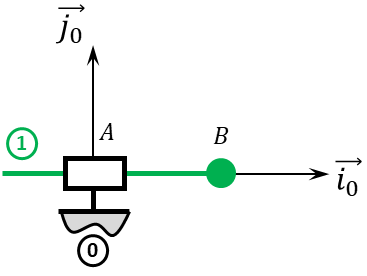
\includegraphics[width=.6\linewidth]{01_T_01}
\end{center}
\fi
\subparagraph{}
\textit{Retracer le schéma cinématique pour $\lambda=\SI{10}{mm}$ et $\lambda=-\SI{10}{mm}$.}
\ifprof

\ifcorrection
\else
\textbf{Pas de corrigé pour cet exercice.}
\fi
\else
\fi

\ifprof
\else
\begin{flushright}
\footnotesize{Corrigé  voir \ref{B2:12:01}.}
\end{flushright}%
\fi